%# -*- coding:utf-8 -*-
%!TEX root = ../thesis.tex
%%==================================================
%% chapter02.tex for SJTU Master Thesis
%% Encoding: UTF-8
%%==================================================
\newcommand\bu{\bm{u}}
\newcommand\bx{\bm{x}}


%\newcommand{\tabincell}[2]{\begin{tabular}{@{}#1@{}}#2\end{tabular}}


\chapter{水下机器人系统模型 }

% 参考的资料fossen的书\\
%  remus的硕士论文\\
% 欠驱动与全驱动机器人的介绍russ tedrake http://underactuated.csail.mit.edu/underactuated.html

\label{chap:Theory}
% 2.1 引言
% 2.2 运动系统数学描述
% 2.2.1 水下机器人的坐标系统
% 2.2.2 水下机器人的运动动力学模型
% 2.2.3 不同类型的水下机器人模型
% 2.2.3.1 全驱动水下机器人的数学模型
% 2.2.3.2 欠驱动水下机器人的数学模型
% 2.3 推进器布置与推力控制向量
% 2.4 本章小结
\section{引言}
水下机器人可根据设备应用的目标与操控方式的不同通常可以分为自治式水下机器人(AUV)、遥控水下机器人(ROV)。水下机器人的种类不同使得不同的水下机器人在设计开发阶段就着重于不同的水下功用,但这样的划分主要是从功用角度划分,这使得研究者在后续的控制开发中容易忽略动态系统本身的特性,更过多地依赖于控制系统设计。运动学、动力学理论常常被用来分析水下机器人的运动,这种方法无论是AUV还是ROV类型的水下机器人均可使用。水下机器人的运动空间是6自由度的,采用矩阵形式的运动动力学方程可以用于水下机器人的理论分析,但是从现代机器人行业的发展对水下机器人研究带来的挑战的角度,即如何更好利用蕴含在机器人设备中的自然动力学或者系统特性更好地改善控制系统的设计,精确地建立航行器的数学模型代价太高。

根据机器人的控制输入与系统的自由度,机器人控制也会呈现出不同的驱动特性。参考现代机器人(机器鱼、 ASIMO、飞行器)与生物(鱼、鸟类)的在执行任务与获得的运动性能的运动自然性上的强烈差异,机器人(鱼)就像一个不太熟悉自身系统的人(鱼)\cite{russdrakebook}。这是因为过往的机器人控制系统主要采用状态反馈控制的方法,虽然可以让机器人系统追踪上期望轨迹,但是这样的控制不仅需要使用高增益的反馈并耗费较多的能量,还需要设计者对控制理论比较精通。(水下)机器人研究的目标是其实现卓越的动态性能(效率,敏捷性和鲁棒性),这需要研究者意识到利用系统的动态特性来开发控制系统的重要性,而不是消除它们。水下机器人的研究主要就是建立可以利用机器人系统的动力学特性来设计控制系统。

一般而言,根据水下机器人工作的水下空间和推进器的分配布置,水下机器人,尤其是深海工作的无人自治水下机器人,多是控制输入小于系统的自由度。本章为了便于后续的控制建模研究,将水下机器人基于外形划分成为鱼雷型水下机器人和具有复杂外形的水下机器人。两种水下机器人的系统描述都是基于海洋运载器的数学模型,主要从静力学、动力学来描述水下机器人在体坐标系下的力与运动的关系,并通过建立大地坐标系与体坐标系来完成状态量的转换。描述水下机器人的方法有许多种,主要有运动动力学建模法、使用实验数据系统建模法来获取载体系统的数学模型。本章的工作是从利用系统动态和便于模型参数计算的角度对水下机器人进行分类,并演绎水下机器人的运动动力学模型的各个具体形式。结合推进器的空间安装位置,从运动学的角度给出推力分配模型。根据水下机器人运动面的划分,对一般形式的推力分配模型进行演化,但与所要控制的运动而言,有些推进器的布置并不是最合适的。基于控制目标,分析各推进器对每个自由度运动的贡献,提出推力控制向量,以便定义单个推进器对各自由度的力学影响。结合ROV的姿态控制,将PID控制器与推力控制向量结合,以优化推力的分配,改善控制性能。

\section{运动系统数学描述 }

水下机器人系统的数学建模涉及到运动学、动力学、静力学的有关知识。运动学是涉及水下机器人的有关量表达以及运动转换的几何方面研究。静力学主要关于水下机器人处于静止或者稳定状态的力学平衡,动力学主要是与本体有关加速运动的力学分析。本部分首先介绍水下机器人的六个自由度的运动学动力学模型以及关键项,分别建立水下机器人的刚体平动、转动的模型以及非线性航行器模型。为了便于引入后续的系统辨识和模型计算章节,重点介绍两种不同机器人的数学模型。

\begin{figure}[!htp]
\centering
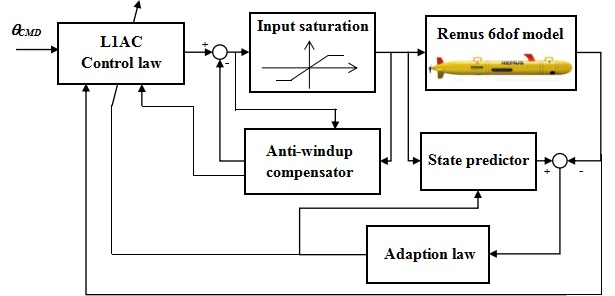
\includegraphics[width=10cm,height=9cm]{figure/chap2/F1.eps}
%\captionsetup{justification=centering}
% \caption{水下运载器坐标示意图}
% \label{paper_f11}
\label{fig:chap2:F1}
\bicaption[fig:chap2:F1]{水下运载器坐标示意图}{水下运载器坐标示意图} {Fig.}{Underwater vehicle frames}
\end{figure}

\begin{table}[!hpb]
\centering
\label{tab:chap2:notation}
\bicaption[tab:chap2:notation]{水下机器人符号量示意}{水下机器人符号量示意}{Table}{ Notations for Underwater vehicle\cite{fossen1994guidance}}
\begin{tabular}{cccc}
\toprule
      & Position \& Angles   &  Linear \& Angular Velocities  & Forces \& Moments \\
Coordinate & E-frame & B-frame & B-frame \\ \midrule
Surge & $X$      &  $u$ & $F_X$ \\
Sway  & $Y$      &  $v$ & $F_Y$ \\
Heave & $Z$      &  $w$ & $F_Z$ \\
Roll  & $\varphi$&  $p$ & $M_K$ \\
Pitch & $\theta$ &  $q$ & $M_M$ \\
Yaw   & $\psi$   &  $r$ & $M_N$ \\
\bottomrule
\end{tabular}
\end{table}

\subsection{水下机器人的运动学 }

在水下机器人中,通常会采用两个坐标系来描述水下机器人本体的运动,即体坐标系(B-frame)和惯性坐标系(E-frame),如图所示\ref{fig:chap2:F1}。其中,体坐标系统(B-frame)的坐标原点$O$位于水下机器人本体的几何中心上,体坐标系的x轴的正向为水下机器人的前进方向,体坐标系的y轴指向水下机器人的右侧,体坐标系的定义符合右手定义,因此z轴指向水下机器人的正下方。惯性坐标系(E-frame),也常被称为大地坐标系,大地坐标系的定义可以参考海军建筑师和船舶工程师学会(SNAME)在1950年建立的坐标系规范,其中大地坐标系常被用来描述水下机器人的运动任务以及导航位置,该坐标系的X、Y、Z分别指向北(North)、东(East)、地心(Down),因此大地坐标系也被称为NED-frame\cite{fossen1994guidance}。考虑后面水下机器人建模的复杂性,为了方便,模型是在体坐标系内建立的,而水下机器人各运动量可以参见表\ref{tab:chap2:notation}。机器人的方位姿态和位置$\bm \eta$是在E-frame内定义,速度量$\bm \nu$是在B-frame中表示的,水下机器人受到的力和力矩$\bm \tau$ 也是在B-frame表示,如公式\ref{eq:chap2:1}。在海洋运载器的导航与控制系统中,运载器的姿态是使用欧拉角(或四元数)来表示的,本章中为了便于后续的使用,也将会介绍体坐标系运动学方程相对于惯性坐标系的转换关系。在表\ref{tab:chap2:notation}中,水下机器人的六个自由度都被反映并示意出来,Surge是纵荡,Sway是横荡,Heave是垂荡,Roll是横滚,Pitch是俯仰,Yaw是偏航。所有的位置、姿态、线速度、角速度以及力、力矩都分别与这六个自由度对应。



\begin{equation}
\centering
\label{eq:chap2:1}
\begin{aligned}
 {\bm{\eta}}  &= {[X,Y,Z,\varphi ,\theta ,\psi ]^T} \\
 {\bm{\nu}} &= {[u,v,w,p,q,r]^T} \\
 {\bm{\tau}_{RB}} &= {[ \sum {F_X}, \sum {F_Y}, \sum {F_Z}, \sum {M_K}, \sum {M_M}, \sum {M_N}]^T}\\
 \end{aligned}
 \end{equation}
 其中,为了便于进行姿态和位置计算,定义如下向量:
 \begin{equation*}
 \centering
 \label{eq:chap2:2}
 \begin{array}{l}
 {{\bm{\eta}} _1} = {[X,Y,Z]^T} \\
 {{\bm{\eta}} _2} = {[\varphi ,\theta ,\psi ]^T}\\
 {{\bm{\nu}} _1}= {[u,v,w]^T}\\
 {{\bm{\nu}} _2}= {[p,q,r]^T}\\
 {{\bm{\tau}}_1} = {[ \sum {F_X}, \sum {F_Y}, \sum {F_Z}]^T}\\
 {{\bm{\tau}}_2} = {[ \sum {M_K}, \sum {M_M}, \sum {M_N}]^T}\\
 \end{array}
 \end{equation*}



平移运动的速度向量在体坐标系和惯性坐标系的转换如下公式\ref{eq:chap2:3}所示:

\begin{equation}
\centering
\label{eq:chap2:3}
\left[ {\begin{array}{*{20}{c}}
   {\dot X}  \\
   {\dot Y}  \\
   {\dot Z}  \\
\end{array}} \right] =
 {{\bm{J}}_{1}(\bm{\eta}_{2})}
\left[ {\begin{array}{*{20}{c}}
   u  \\
   v  \\
   w  \\
\end{array}} \right]
\end{equation}
其中,
\begin{equation*}
\centering
\label{eq:chap2:4}
{{\bm{J}}_{1}(\bm{\eta} _{2})} =
\left[
{\begin{array}{*{20}{c}}
   {{\mathop{\rm c}\nolimits}  \psi  c \theta  } & { - s \psi  c \varphi   + c \psi  s \varphi  s \theta  } & {s \psi  s \varphi   + {\mathop{\rm c}\nolimits}  \psi  c \varphi  s \theta  }  \\
   {s \psi  c \theta  } & {c \psi  c \varphi   + s \psi  s \varphi  s \theta  } & { - c \psi  s \varphi   + s \psi  c \varphi  s \theta  }  \\
   { - s \theta  } & {c \theta  s \varphi  } & {c \theta  c \varphi  }  \\
\end{array}}
\right]
\end{equation*}
\\
在上述公式以及后面的方程中,为了描述方便,定义 $ c= cos(·)$ ,  $s = sin(·)$, $t = tan(·)$。需要注意的是,${{\bm{J}}_{1}(\bm{\eta} _{2})}$ 是正交矩阵,因此,

\begin{equation}
\label{eq:chap2:5}
({{\bm{J}}_{1}(\bm{\eta} _{2})})^{-1} = ({{\bm{J}}_{1}(\bm{\eta} _{2})})^T
\end{equation}

旋转运动的速度向量在体坐标系和惯性坐标系的转换如下,如下公式所示\ref{eq:chap2:6}:

\begin{equation}
\label{eq:chap2:6}
\left[ {\begin{array}{*{20}{c}}
   \dot \varphi   \\
   \dot \theta   \\
   \dot \psi   \\
\end{array}} \right] = {\bm{J}_2(\bm{\eta}_2)}
\left[ {\begin{array}{*{20}{c}}
   p  \\
   q  \\
   r  \\
\end{array}} \right]
\end{equation}
其中,${\bm{J}_2(\bm{\eta}_2)}$ 的具体表示如下

\begin{equation*}
\centering
\label{eq:chap2:7}
{\bm{J}_2(\bm{\eta}_2)} =
 \left[ {\begin{array}{*{20}{c}}
   1 & {{\mathop{\rm s}\nolimits}  \varphi  {\mathop{\rm t}\nolimits}  \theta  } & {{\mathop{\rm c}\nolimits}  \varphi  {\mathop{\rm t}\nolimits}  \theta  }  \\
   0 & {{\mathop{\rm c}\nolimits}  \varphi  } & { - {\mathop{\rm s}\nolimits}  \varphi  }  \\
   0 & {{\mathop{\rm s}\nolimits}  \varphi  /{\mathop{\rm c}\nolimits}  \theta  } & {{\mathop{\rm c}\nolimits}  \varphi  /{\mathop{\rm c}\nolimits}  \theta  }  \\
\end{array}} \right]
\end{equation*}

需要注意的是,${\bm{J}_2(\bm{\eta}_2)}$ 的公式并不适用与俯仰角度 $\theta$ 接近+90度或者-90度的情况。 对于水下机器人的运动描述,这个问题并不会影响使用,因为实际的使用水下机器人几乎不会到达这个奇点。如果是需要对极端情况的俯仰角度进行建模研究,也可以使用四元数或者罗德里格斯参数来实现\cite{fossen1994guidance}。

通过使用公式\ref{eq:chap2:3}和\ref{eq:chap2:6}的线速度转换矩阵与旋转变换矩阵,可以得到水下机器人体坐标系与惯性坐标系之间的运动学关系:

\begin{equation}
\label{eq:chap2:8}
\dot{\bm{\eta}}= \bm{J(\bm{\eta}_2)}   \dot{\bm{\nu}}
\end{equation}

可以发现$\bm{J(\bm{\eta}_2)}$ 是关于 $\bm{\eta}_2$ 的函数,其具体数学描述如下:

\begin{equation}
\label{eq:chap2:9}
\bm{J(\bm{\eta}_2)} = \begin{bmatrix}
 {\bm{J}_1(\bm{\eta}_2)}  &   \bm{0}_{3 \times 3}\\
 \bm{0}_{3 \times 3}      &  {\bm{J}_2(\bm{\eta}_2)}
\end{bmatrix}
\end{equation}

通过使用上面的运动学定义与相关量的转换,可以继续水下机器人的动力学建模工作。

\subsection{水下机器人的动力学模型  }
由于航行器所受到刚体动力学与流体动力学作用到本体上具有同时性,可以根据线性系统的等效叠加原理进行动力学建模\cite{lamb1932hydrodynamics}。因此,将水下机器人的动力学建模主要分为刚体动力学建模与流体动力学建模。

\subsubsection{航行器的刚体动力学 }

在本部分进行的刚体动力学的研究是不考虑水对运载器的影响,且在体坐标系上使用牛顿定律、欧拉运动定律进行分析。因此,需建立两个假设:一是水下机器人被假设为一个理想的刚体,其受到的所有力学作用等效为一个合外力(矩);二是认为定义在地球上的惯性坐标系不受地球运动产生的力影响\cite{prestero2001verification}。刚体动力学的研究也是从平动和旋转运动两个方面展开。

在进行研究前,需要定义水下机器人在体坐标系的重心和浮心的位置,如下所示:
\begin{equation}
\label{eq:chap2:10}
\begin{aligned}
{\bm{r}}_{G} &= [ x_G,  y_G,  z_G ]^T  \\
{\bm{r}}_{B} &= [ x_B,  y_B,  z_B ]^T  \\
\end{aligned}
\end{equation}

考虑到体坐标系的原点不位于水下机器人的几何中心上,具有一般性。因此水下航行器的6自由度的刚体动力学方程如下:
\begin{equation}
\label{eq:chap2:11}
 %\begin{array}{l}
 \begin{aligned}
 m\left[ {\dot u - vr + wq - {x_G}({q^2} + {r^2}) + {y_G}(pq - \dot r) + {z_G}(pr + \dot q)} \right] &= \sum {{F_X}}  \\
 m\left[ {\dot v - wp + ur - {y_G}({r^2} + {p^2}) + {z_G}(qr - \dot p) + {x_G}(qp + \dot r)} \right] &= \sum {{F_Y}}  \\
 m\left[ {\dot w - uq + vp - {z_G}({q^2} + {p^2}) + {x_G}(rp - \dot q) + {y_G}(rq + \dot p)} \right] &= \sum {{F_Z}}  \\
 {I_x}\dot p + ({I_z} - {I_y})qr -(\dot r + pq)I_{xz}+(r^2-q^2)I_{yz}+(pr-\dot q)I_{xy}\\
               + m[{y_G}(\dot w - uq + vp) - {z_G}(\dot v - wp + ur)] &= \sum {{M_K}}  \\
 {I_y}\dot q + ({I_x} - {I_z})rp -(\dot p + qr)I_{xy}+(p^2-r^2)I_{xz}+(qp-\dot r)I_{yz}\\
               + m[{z_G}(\dot u - vr + wq) - {x_G}(\dot w - uq + vp)] &= \sum {{M_M}}  \\
 {I_z}\dot r + ({I_y} - {I_x})pq -(\dot q + rp)I_{yz}+(q^2-p^2)I_{xy}+(rq-\dot p)I_{xz}\\
               + m[{x_G}(\dot v - wp + ur) - {y_G}(\dot u - vr + qw)] &= \sum {{M_N}}  \\
 \end{aligned}
 %\end{array}
 \end{equation}
式\ref{eq:chap2:11}中$m$ 是水下机器人的质量,公式的前三个方程表示平移运动,后三个方程表示旋转运动。

将上述方程表达成更加紧凑的矩阵形式:

\begin{equation}
\label{eq:chap2:12}
\bm{M_{RB}} {\dot{\bm{\nu}}} + \bm{C_{RB}}(\bm{\nu}){\bm{\nu}} =  {\bm{\tau}_{RB}}
\end{equation}
公式\ref{eq:chap2:12}即是水下机器人的刚体动力学的一般形式,其中${\bm{\tau}_{RB}}$是外部的力、力矩的合向量。刚体惯性质量矩阵是唯一不随时间变化的,并且具有如下属性:$\bm{M_{RB}} = \bm{M_{RB}}^T > \bm{0}$。$\bm{M_{RB}}$的具体表达见公式\ref{eq:chap2:13}, $\bm{\tau_{RB}}$ 在公式\ref{eq:chap2:1}已经被定义。
\begin{equation}
\label{eq:chap2:13}
\begin{aligned}
\bm{M_{RB}} &= \begin{bmatrix}
               {m {\bm{I_{3 \times 3}} }} & {-m {\bm{S_{r_G}} } }   \\
                 m {\bm{S_{r_G}} }         &  \bm{I_0} \\
               \end{bmatrix}
            &= \begin{bmatrix}
                   m & 0       &  0    & 0        & m z_G   & -m y_G     \\
                   0 & m       &  0    & -m z_G   & 0       & m x_G      \\
                   0 & 0       &  m    &  m y_G   & -m x_G  & 0          \\
                   0 &  -m z_G & m y_G &  I_x     & -I_{xy} & -I_{xz}    \\
               m z_G &   0     & -m x_G& -I_{yx}  & I_y     & -I_{yz}    \\
              -m y_G &  m x_G  &  0    & -I_{zx}  & -I_{zy} & I_z        \\
               \end{bmatrix}
\end{aligned}
\end{equation}
式\ref{eq:chap2:13}中,${\bm{I_{3 \times 3}}}$为单位矩阵,$\bm{I_0}$ 是惯性张量矩阵,$\bm{S_{r_G}}$是斜对称矩阵。

式\ref{eq:chap2:12}中, ${\bm{C_{RB}}(\bm{\nu})}$ 是科氏力-离心力矩阵,  它包括科氏力向量项与离心力向量项, 是斜对称矩阵, 也具有如下性质:${\bm{C_{RB}}(\bm{\nu})}= - {\bm{C_{RB}}(\bm{\nu})}^T$,具体可参考附录定理\ref{app_A:thm:1}的惯性矩阵的科氏力-离心力矩阵参数化定理。

${\bm{C_{RB}}(\bm{\nu})}$ 的具体定义参数化如下:
% \begin{equation}
% \bm{C_{RB}}(\bm{\nu}) {\buildrel \Delta \over =}
% \begin{bmatrix}
% 0 & 0 & 0  & m(y_G q + z_G r) & -m(x_G q - w)   & -m(x_G r + v)   \\
% 0 & 0 & 0  & -m(y_G p +w)     & m(z_G r +x_G p) & -m(y_G r - u)  \\
% 0 & 0 & 0  & -m(z_G p - v)    & -m(z_G q + u)   & m(x_G p + y_G q)  \\
% -m(y_G q + z_G r) & m(y_G p+w)   & m(z_G p - v) &0  & -I_{yz}q-I_{xz}p+I_z r &  I_{yz}r +I_{xy}p - I_y q          \\
% m(x_G q - w) & -m(z_G r + x_G p)  &  m(z_G q+u) & I_{yz}q+I_{xz}p - I_z r & 0 & -I_{xz}r - I_{xy}q + I_{x}p \\
% m(x_G r + v) &  m(y_G r - u) & -m(x_G p + y_G q) & -I_y r - I_{xy}p +I_y q & I_{xz}r+I_{xy}q-I_x p &  0 \\
% \end{bmatrix}
% \end{equation}
\begin{multline}
\label{eq:chap2:14}
%\begin{aligned}
\bm{C_{RB}}(\bm{\nu})
{\buildrel \Delta \over =}
% \begin{bmatrix}
%   0 & 0  \\
%   0 & 0  \\
% \end{bmatrix}\\
% =
  \left[\begin{array}{ccc}
0 & 0 & 0 \\
0 & 0 & 0 \\
0 & 0 & 0 \\
-m(y_G q + z_G r) & m(y_G p+w)   & m(z_G p - v) \\
m(x_G q - w) & -m(z_G r + x_G p)  &  m(z_G q+u) \\
m(x_G r + v) &  m(y_G r - u) & -m(x_G p + y_G q) \\
\end{array}\right.\\
\left.\begin{array}{ccc}
  m(y_G q + z_G r) & -m(x_G q - w)   & -m(x_G r + v)   \\
  -m(y_G p +w)     & m(z_G r +x_G p) & -m(y_G r - u)  \\
 -m(z_G p - v)    & -m(z_G q + u)   & m(x_G p + y_G q)  \\
 0  & -I_{yz}q-I_{xz}p+I_z r &  I_{yz}r +I_{xy}p - I_y q   \\
 I_{yz}q+I_{xz}p - I_z r & 0 & -I_{xz}r - I_{xy}q + I_{x}p \\
 -I_y r - I_{xy}p +I_y q & I_{xz}r+I_{xy}q-I_x p &  0 \\
\end{array}\right]
%\end{aligned}
\end{multline}

因此,可以获得水下机器人的矩阵形式刚体动力学,并对各项进行参数化分析。

考虑前面的体坐标系的原点不是位于水下机器人的几何中心上,假设浮心与体坐标系原点重合,则可以获得对角化的惯性张量矩阵:

\begin{equation}
\label{eq:chap2:15}
\bm{I}_0 = \begin{bmatrix}
 I_x  & 0    &  0   \\
 0    & I_y  &  0   \\
 0    & 0    &  I_z \\
\end{bmatrix}
\end{equation}

简化后的运动方程如下:
\begin{equation}
\centering
\label{eq:chap2:16}
\begin{array}{l}
 m\left[ {\dot u - vr + wq - {x_G}({q^2} + {r^2}) + {y_G}(pq - \dot r) + {z_G}(pr + \dot q)} \right] = \sum {{F_X}}  \\
 m\left[ {\dot v - wp + ur - {y_G}({r^2} + {p^2}) + {z_G}(qr - \dot p) + {x_G}(qp + \dot r)} \right] = \sum {{F_Y}}  \\
 m\left[ {\dot w - uq + vp - {z_G}({q^2} + {p^2}) + {x_G}(rp - \dot q) + {y_G}(rq + \dot p)} \right] = \sum {{F_Z}}  \\
 {I_x}\dot p + ({I_z} - {I_y})qr + m[{y_G}(\dot w - uq + vp) - {z_G}(\dot v - wp + ur)] = \sum {{M_K}}  \\
 {I_y}\dot q + ({I_x} - {I_z})rp + m[{z_G}(\dot u - vr + wq) - {x_G}(\dot w - uq + vp)] = \sum {{M_M}}  \\
 {I_z}\dot r + ({I_y} - {I_x})pq + m[{x_G}(\dot v - wp + ur) - {y_G}(\dot u - vr + qw)] = \sum {{M_N}}  \\
 \end{array}
 \end{equation}

\subsubsection{航行器作用力 }

本部分主要从水下机器人的流体力学角度对运载器进行分析,根据刚体动力学模型公式\ref{eq:chap2:12}右侧表示的作用于水下机器人上的外部合力与力矩以及线性叠加原理,合力(矩)的产生原因可以分为如下几类:
一. 流体作用力$\bm{\tau}_{H}$,包括附加质量、流体阻尼力、恢复力(浮力与重力共同作用的静力学分析)。二. 环境干扰力$\bm{\tau}_E$,一般因受到海流、风、波浪环境影响而产生,由于水下机器人所工作的环境主要在深水区域, 因此本章仅考虑海流的力学效应。另外,在水下机器人中水流对水下机器人的影响被视为干扰力,一般通过控制来克制,不过本文对于水流的研究不仅仅处于将水流视为外界的干扰,也在主动地识别流体的特性,主动利用水下环境。在第三章中,会给出关于水流的特性识别的有关研究工作。三. 驱动力$\bm{\tau}$,一般包括推进器、舵片的力学作用。

根据水下机器人受到的外部力(矩)的成因,给出作用力的数学描述如下:
\begin{equation}
\centering
\label{eq:chap2:17}
\bm{\tau}_{RB} = \bm{\tau}_{H} + \bm{\tau}_E +  \bm{\tau}
\end{equation}
\begin{equation}
\label{eq:chap2:18}
\bm{\tau}_{H} = -{\bm{M}_A}{\bm{\dot \nu}} - {\bm{C}_A}(\bm{\nu}) {\bm{\nu}} - \bm{D}(\bm{\nu})\bm{\nu}-\bm{g}({\bm{\eta}})
\end{equation}
式\ref{eq:chap2:17}与式\ref{eq:chap2:18} 共同给出水下航行器受到的外部作用力和力矩的数学模型。

为了便于进行水下机器人建模与控制应用,下面分别给出相关项的参数化矩阵与数学分析。

A. 附加质量项

惯性附加质量$\bm{M}_A$ 是由水下机器人在水中加速运动而产生的水动力。 对于完全没入水中的水下机器人, 在对附加质量$\bm{M}_A $求解时会假设附加质量的系数是恒定不变的,并且不受波浪频率的影响,但是附加质量的某些项却比机器人的本体质量大很多。基于这个假设,流体动能来被用来分析附加质量项,当水下机器人在水中加速运动时,机器人头部的流体会因前进运动而向机器人后方移动,这样的移动必定会耗费的能量。附加质量项定义如下:

\begin{equation}
\centering
\label{eq:chap2:19}
\begin{aligned}
\bm{M}_{A}  &= \begin{bmatrix}
                 \bm{A}_{11}   &  \bm{A}_{12}   \\
                 \bm{A}_{21}   &  \bm{A}_{22}   \\
               \end{bmatrix}                    \\
            &=-\begin{bmatrix}
 X_{\dot u} &  X_{\dot v} &  X_{\dot w} &  X_{\dot p} &  X_{\dot q} &  X_{\dot r} \\
 Y_{\dot u} &  Y_{\dot v} &  Y_{\dot w} &  Y_{\dot p} &  Y_{\dot q} &  Y_{\dot r} \\
 Z_{\dot u} &  Z_{\dot v} &  Z_{\dot w} &  Z_{\dot p} &  Z_{\dot q} &  Z_{\dot r} \\
 K_{\dot u} &  K_{\dot v} &  K_{\dot w} &  K_{\dot p} &  K_{\dot q} &  K_{\dot r} \\
 M_{\dot u} &  M_{\dot v} &  M_{\dot w} &  M_{\dot p} &  M_{\dot q} &  M_{\dot r} \\
 N_{\dot u} &  N_{\dot v} &  N_{\dot w} &  N_{\dot p} &  N_{\dot q} &  N_{\dot r} \\
              \end{bmatrix}
\end{aligned}
\end{equation}
式中,$\bm{A}_{11}$, $ \bm{A}_{12}$, $\bm{A}_{21}$,$\bm{A}_{22}$均为$3 \times 3$矩阵,其余量为水下机器人的与加速度有关的流体动力学参数。

由于附加质量$\bm{M}_A$ 产生的科氏力-离心力, 水下机器人在做旋转运动的时候也会因加速而消耗能量。 因此,给出斜对称矩阵${\bm{C}_A}\left( \bm{ \nu}  \right)$的定义:
\begin{equation}
\centering
\label{eq:chap2:20}
{\bm{C}_A}\left( \bm{ \nu}  \right) = \left[ {\begin{array}{*{20}{c}}
   0 & 0 & 0 & 0 & { - {a_3}} & {{a_2}}  \\
   0 & 0 & 0 & {{a_3}} & 0 & { - {a_1}}  \\
   0 & 0 & 0 & { - {a_2}} & {{a_1}} & 0  \\
   0 & { - {a_3}} & {{a_2}} & 0 & { - {b_3}} & {{b_2}}  \\
   {{a_3}} & 0 & { - {a_1}} & {{b_3}} & 0 & { - {b_1}}  \\
   { - {a_2}} & {{a_1}} & 0 & { - {b_2}} & {b1} & 0  \\
\end{array}} \right]
\end{equation}

其中,\begin{equation*}
\label{eq:chap2:21}
\begin{array}{l}
 {a_1} = {X_{\dot u}}u + {X_{\dot v}}v + {X_{\dot w}}w + {X_{\dot p}}p + {X_{\dot q}}q + {X_{\dot r}}r \\
 {a_2} = {X_{\dot v}}u + {Y_{\dot v}}v + {Y_{\dot w}}w + {Y_{\dot p}}p + {Y_{\dot q}}q + {Y_{\dot r}}r \\
 {a_3} = {X_{\dot w}}u + {Y_{\dot w}}v + {Z_{\dot w}}w + {Z_{\dot p}}p + {Z_{\dot q}}q + {Z_{\dot r}}r \\
 {b_1} = {X_{\dot p}}u + {Y_{\dot p}}v + {Z_{\dot p}}w + {K_{\dot p}}p + {K_{\dot q}}q + {K_{\dot r}}r \\
 {b_2} = {X_{\dot p}}u + {Y_{\dot q}}v + {Z_{\dot q}}w + {K_{\dot q}}p + {M_{\dot q}}q + {M_{\dot r}}r \\
 {b_3} = {X_{\dot r}}u + {Y_{\dot r}}v + {Z_{\dot r}}w + {K_{\dot r}}p + {M_{\dot r}}q + {N_{\dot r}}r \\
 \end{array}
 \end{equation*}

一般而言,6自由度的水下机器人在水下高速航行是具有强非线性且复杂耦合性。然而,在许多水下机器人中,例如ROV,如果其运动的速度较低,且拥有三个对称平面,这时就可以忽略附加质量项矩阵内不在对角线上的元素。故惯性附加质量矩阵$\bm{M}_A$和$\bm{C}_A$可以简化成如下形式:
\begin{equation}
\centering
\label{eq:chap2:22}
\bm{M}_A = -diag\{X_{\dot u},Y_{\dot v},Z_{\dot w},K_{\dot p},M_{\dot q},N_{\dot r}\}
\end{equation}
\begin{equation}
\label{eq:chap2:23}
\centering
\bm{C}_A  = \begin{bmatrix}
 0           &0            &0               &0                  &-Z_{\dot w} w   & Y_{\dot v} v\\
 0           &0            &0               &Z_{\dot w}w        &0               &-X_{\dot u}u\\
 0           &0            &0               &-Y_{\dot v}v       & X_{\dot u} u   &   0    \\
 0           & -Z_{\dot w}w & Y_{\dot v}v   &  0                & -N_{\dot r}r   & M_{\dot q}q\\
 Z_{\dot w}w &0            &-X_{\dot u}u    & N_{\dot r}r       & 0              &-K_{\dot p}p \\
 -Y_{\dot v}v& X_{\dot u}u &0               &-M_{\dot q}q       & K_{\dot p}p    & 0\\
\end{bmatrix}
\end{equation}
虽然获得的附加质量矩阵是简化的,但在实际使用是,这种近似方法的估计效果良好,这是因为对角线上的元素远大于非对线上的元素。对于超小型的水下机器人,因本体质量较小,且速度足够小,一般可以将$\bm{C}_A$忽略。


B. 阻尼项

公式\ref{eq:chap2:18}中的流体阻尼项的出现主要原因有本体运动而带来的势流阻尼;有机器人本体的表面因运动而产生摩擦阻尼,该阻尼主要与表面积有关;有水下机器人运功因为兴波耗费能量而产生的阻尼;有因流体流过机器人时会产生漩涡而引起机器人的振动而耗散能量的阻尼。总流体动力学阻尼矩阵可以写成这些分量的总和:
\begin{equation}
\label{eq:chap2:24}
\bm{D}({\bm{\nu}})  {\buildrel \Delta \over =} \bm{D}_P(\bm{\nu})+\bm{D}_S(\bm{\nu})+\bm{D}_W(\bm{\nu})+\bm{D}_M(\bm{\nu})
\end{equation}
式中,$\bm{D}_P(\bm{\nu})$ 是势流阻尼项,$\bm{D}_S(\bm{\nu})$是摩擦阻尼项, $\bm{D}_W(\bm{\nu})$是兴波阻尼,$\bm{D}_M(\bm{\nu})$ 是漩涡脱落阻尼。

在水下机器人中,$\bm{D}_P(\bm{\nu})$相比于别的耗散项如粘性阻尼都是可以忽略的。

考虑运载器的运动是低频的,层流边界层产生的线性表皮摩擦会很重要。另外由于线性摩擦对于湍流边界层也有影响,因此通常认为$\bm{D}_W(\bm{\nu})$ 是重要的,且是二次非线性表皮摩擦。

水下机器人多工作于深海,而在靠近海表面运动才会有$\bm{D}_M(\bm{\nu})$产生。因此,在水下机器人中一般会忽略 兴波阻尼。

水是粘性流体,因此由于摩擦力的存在这样的系统能量不会保持。漩涡脱落阻尼常采用莫里森公式来计算,而且在经验计算中莫里森公式常被用来计算水下机器人的流体阻尼:
\begin{equation}
\label{eq:chap2:25}
f(U)=-\frac{1}{2} \rho C_{D}(R_n)A \left |U \right | U
\end{equation}
式中,$U$ 是机器人的前进速度;$A$ 是运动方向的投影截面面积;$C_{D}(R_n)$ 是阻力系数;$\rho$是流体密度,一般流体为水。阻尼系数是和雷诺数有关的$R_n$,雷诺数的计算可以参考\cite{fossen1994guidance}。

一般而言,水下机器人的高速6自由度的运动是强非线性的和耦合的。然而,假如水下机器人有三个对称面,可以做一个线性近似,这样二阶及以上的项就可以忽略。这表明$\bm{D}(\bm{\nu})$的对角线上只有线性的和二次阻尼项。 公式如下:
\begin{equation}
\label{eq:chap2:26}
\begin{aligned}
\bm{D}(\bm{\nu})= &- diag\{ X_u,Y_v,Z_w,K_p,M_q,N_r\}   \\
                  &- diag\{ X_{u\left|u\right|} \left|u\right|, Y_{v\left|v\right|} \left|v\right| , Z_{w\left|w\right|} \left|w\right|, K_{p\left|p\right|} \left|p\right| , M_{q \left| q \right|} \left| q \right|, N_{r \left| r \right|} \left| r \right|  \}
\end{aligned}
\end{equation}
即水下机器人的阻尼项的计算可以总结为线性阻尼和非线性阻尼,其中,非线性的成分会占比更大。

C. 恢复力和力矩

水下机器人中,重力和浮力统称为恢复力。重力的作用点在水下机器人的重心上$\bm{r}_G$ 上, 而浮力的作用点在浮心$\bm{r}_B$ 上。一般而言,水下机器人的重心和浮心是不重合的,并且水下机器人由于在水中的姿态是不断变化的,这样,由于浮力和重力产生力矩也是不断变化的。使用欧拉角在惯性坐标系下给出恢复力和力矩的数学公式:
\begin{equation}
\centering
\label{eq:chap2:27}
\bm{g}(\bm {\eta} ) = \left[ {\begin{array}{*{20}{c}}
   {\left( {W - B} \right)s\theta }  \\
   { - \left( {W - B} \right)c\theta s\varphi }  \\
   { - \left( {W - B} \right)c\theta c\varphi }  \\
   { - \left( {{y_G}W - {y_G}B} \right)c\theta c\varphi  + \left( {{z_G}W - {z_B}B} \right)c\theta s\varphi }  \\
   {\left( {{z_G}W - {z_B}B} \right)s\varphi  + \left( {{x_G}W - {x_B}B} \right)c\theta c\varphi }  \\
   { - \left( {{x_G}W - {x_B}B} \right)c\theta s\varphi  - \left( {{y_G}W - {y_B}B} \right)s\theta }  \\
\end{array}} \right]
\end{equation}
式中,$W$是水下机器人的重力,$B$是浮力。水下机器人中浮力与重力配置会因为水下机器人的类型不同而有所差异,一般ROV中会采用中性浮力,即$W=B$,如BLUEROV。在AUV中,如REMUS-100 AUV中的重力会略小于浮力,这样会使得水下机器人在水里是非稳态系统。这给水下机器人的控制带来了一定的困难。另外,为了减少水下机器人在水里的能量消耗,在设计时也会有重力大于浮力的情况,这种机器人称为重潜于水型水下机器人,多为水下无人机或者水下滑翔机。

D. 驱动器模型

水下机器人的驱动器类型大都是基于流体力学的而设计的,常用的驱动器一般有推进器、控制舵片。水下机器人的驱动器产生力和力矩与水下机器人的固定位置有关,并且驱动器对于水下机器人的各个自由度的影响度也各不相同,将在后面的推力布置部分进行详细讨论。

D.1 螺旋桨模型

对于水下机器人的推进器这种形式,既要描述推进器的布置形式,也要描述单个推进器的数学模型,本部分内容以螺旋桨的推力模型为主。推进器的模型是非线性的,它与水下机器人的航行速度和推进器的转速都有关。为了描述推进器螺旋桨航速和转速的共同作用,给出的推进器的模型如下:
\begin{eqnarray}
\label{eq:chap2:28}
T&=& \rho D^4 K_T (J_0)\|n\| n \\
J_0 &=& \frac{V_a}{nD}\\
K_T&=&\alpha_1 + \alpha_2 \frac{V_a}{nd}
\end{eqnarray}
式中,$K_T$ 是推力系数,$J_0$是流速影响系数。

在ROV中,推进器的推力一般是通过进行敞水实验测定,航向前进速度常被定义为零。推进器的测试台的上配置使用多是S型拉压传感器来测定推进器的正反推力如图\ref{fig:chap2:F2}。推进器也会产生扭矩,在ROV中,推进器一般是成对布置,并且正向推进时的,叶片旋转方向相反,从而抵消推进器的扭矩。因此,推进器的模型就简化成二次非线性表达形式:

\begin{equation}
\label{eq:chap2:29}
T = \alpha_T \left|n\right| n
\end{equation}
式中,$\alpha_T$为敞水推力系数。

\begin{figure}
\label{fig:chap2:F2}
\centering
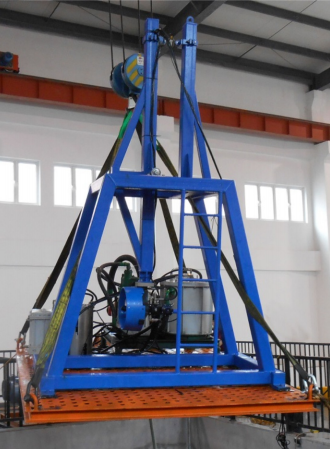
\includegraphics[width = 6cm]{figure/chap2/propellerTest.png}
\bicaption[fig:chap2:F2]{推进器测试台}{推进器测试台}{Fig.}{Test platform for propeller\cite{Huo2016Impulse}}
\end{figure}
本部分建立的推进器螺旋桨的模型描述的是推进器的转速与推力间的关系,但实际中使用的推进器根据推进器采用的驱动方案的不同,推进器的控制输入也不是转速的。液压马达推进器有定量马达和变量马达,电动推进器有无刷直流电机驱动、也有有刷直流电机驱动的方案。因此在实际的应用中可以采用参数辨识方法来确定驱动控制信号与实际推力的关系与系数\cite{wu2016parametric}。

D.2 控制面舵片

安装有控制面舵片的机器人,当航行器在水中前进时,如果舵片与前进方向之间有攻角,舵片上下面会有压力差,产生上升或下降力矩。舵片产生的力矩是水下机器人本体与舵片的共同作用,具有强耦合性与非线性。在确定舵片的力学模型时,一般是采用经验法,与鱼雷数据相对比\cite{bottaccini1954stablity,John1978Methods,Borst1985Fluid}。 另外, 也可以使用实际水下机器人的运行数据来辨识舵片的力学模型,如Hoerner估计方法\cite{Borst1985Fluid}。在后面的水下机器人中使用的舵片就是基于此法建立的模型。

\subsubsection{6自由度水下机器人模型 }

本研究采用的水下机器人的模型是由Fossen提出的非线性海洋运载器模型,该模型是在体坐标系B-frame下将刚体动力学模型公式\ref{eq:chap2:12}与外部合力和力矩模型公式\ref{eq:chap2:17}合并,并结合运动学方程公式\ref{eq:chap2:8}得到水下机器人的模型公式如下\cite{fossen1994guidance}:
\begin{equation}
\label{eq:chap2:30}
\begin{aligned}
\bm{M} \dot {\bm{\nu}} + \bm{C}(\bm{\nu}) \bm{\nu}&
+ \bm{D}(\bm{\nu}) \bm{\nu} + \bm{g}(\bm{\eta}) = \bm{\tau}_E +  \bm{\tau}\\
&\dot{\bm{\eta}}= \bm{J(\bm{\eta}_2)}   \dot{\bm{\nu}}
\end{aligned}
\end{equation}
式中,$\bm{M} = \bm{M}_{RB} +\bm{M}_A$ ; $\quad \bm{C}(\bm{\nu}) =  \bm{C}_{RB}(\bm{\nu}) +  \bm{C}_{A}(\bm{\nu})$。$\bm{M}_A $ 是水下机器人在水中加速而产生附加质量。$\bm{C}_{A}(\bm{\nu})$ 是由于科氏力-离心力作用产生的附加质量。$\bm{D}(\bm{\nu})$ 是阻尼矩阵。$\bm{g}(\bm{\eta})$ 是恢复力与力矩。

假设$\bm{J}(\bm{\eta})$是非奇异矩阵,那么可以获得水下机器人在惯性坐标系下的运动学模型:
\begin{equation}
\label{eq:chap2:31}
\bm{M}_{\bm{\eta}}{\ddot {\bm{\eta}}} +\bm{C}_{\bm{\eta}}(\bm{\nu},\bm{\eta}) {\dot {\bm{\eta}}} + \bm{D}_{\bm{\eta}} (\bm{\nu},\bm{\eta}) {\dot {\bm{\eta}} }+\bm{g}_{\bm{\eta}}(\bm{\eta}) = \bm{\tau}_{\bm{\eta}}+\bm{\tau}_{\bm{\eta}E}
\end{equation}
式中,
\begin{eqnarray}
\label{eq:chap2:32}
\bm{M}_{\bm{\eta}} &=& \bm{J}^{-T}(\bm{\eta})\bm{M}\bm{J}^{-1}(\bm{\eta})\\
\bm{C}_{\bm{\eta}}(\bm{\nu},\bm{\eta}) &=& \bm{J}^{-T}(\bm{\eta})[\bm{C}(\bm{\nu})-\bm{M}\bm{J}^{-1}(\bm{\eta})\bm{J}(\bm{\eta})] \bm{J}^{-1}(\bm{\eta})\\
\bm{D}_{\bm{\eta}} (\bm{\nu},\bm{\eta})&=& \bm{J}^{-T}(\bm{\eta})\bm{D}\bm{J}^{-1}(\bm{\eta})  \\
\bm{g}_{\bm{\eta}}(\bm{\eta}) &=& \bm{J}^{-T}(\bm{\eta}) \bm{g}(\bm{\eta})  \\
\bm{\tau}_{\bm{\eta}} &=& \bm{J}^{-T}(\bm{\eta}) \bm{\tau}\\
\bm{\tau}_{\bm{\eta}E} &=& \bm{J}^{-T}(\bm{\eta})\bm{\tau}_{E}
\end{eqnarray}


\subsection{不同类型的水下机器人模型 }

水下机器人在不同的状态时,系统就会呈现出不同的动力学特性。在本章中,对水下机器人进行的系统描述是水下机器人完全处于水中,且在水中不受外力干扰。根据水下机器人的外形不同,且为便于水下机器人进行模型参数计算时能够提出一套系统的方法,下面主要对具有非初等几何外形的水下机器人和具有鱼雷外形的水下机器人进行系统描述。

\begin{figure}
\centering
\includegraphics[width=12cm,height=12cm]{figure/chap2/F6.eps}
%\captionsetup{justification=centering}
\label{fig:chap2:F3}
\bicaption[fig:chap2:F3]{水池试验图}{水池试验图}{Fig.}{Way-points tracking experiments in the water}
\end{figure}

\begin{figure}
\centering
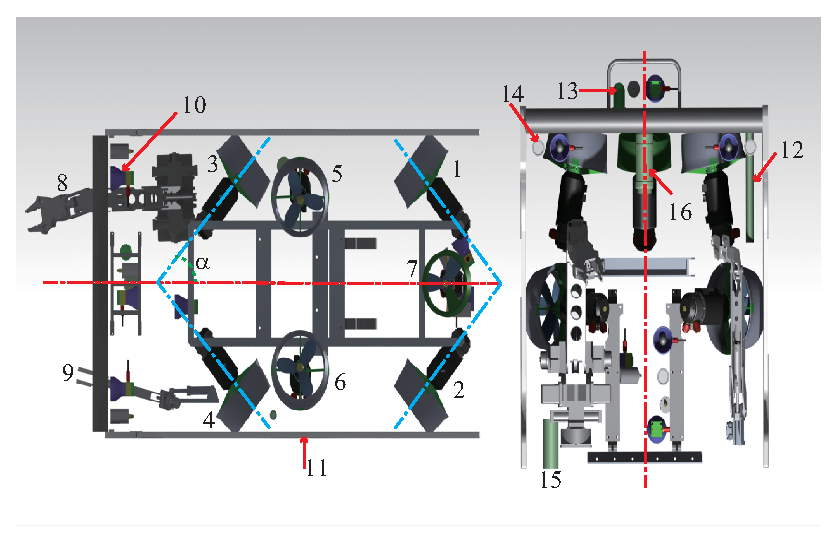
\includegraphics{figure/chap2/F2.eps}
%\captionsetup{justification=centering}
\label{fig:chap2:F4}
\bicaption[fig:chap2:F4]{ROV的分配布置标识图}{ROV的分配布置标识图}{Fig.}{Layout for components of ROV, where 1-7 indicate the position of propellers; 8 and 9 are manipulators used; 10 denotes underwater light; 11 stands for the main frame of vehicle;  12 signifies the wireless beacon of USBL; 13 stands for signal light; 14 is underwater camera;  15 represents the altimeter; 16 expresses the ADCP}
\end{figure}

\begin{table}[h]
\centering
\label{T2:chap2}
\bicaption[T2:chap2]{3000m ROV 的关键参数}{3000m ROV 的关键参数}{Table}{Critical parameters for 3000m ROV}
\begin{tabular}{cccc}
\toprule
               &Value  &Unit   &Description\\
\midrule
\texttt{L}     &2.48     &m  & Overall length\\
\texttt{W}     &1.4      &m  & Width \\
\texttt{H}     &1.63     &m  & Height \\
\texttt{G}     &1413     &kg & Maximum weight\\
\texttt{P}     &1000     &V  & \tabincell{c}{AC Power supply\\ from workstation}\\
\texttt{D$_{max}$}  &3000 &m  & \tabincell{c}{Maximum depth }\\
\texttt{\emph{u}$_{max}$}&2.5 & m/s & Max velocity\\
\texttt{T}&+120 to —90 & kgf &\tabincell{c}{+120:max forward thrust\\-90:max reverse thrust}\\
\texttt{B$_H$}&\tabincell{c}{X-shape\\ $\alpha$=45} & degree & \tabincell{c}{Horizontal propeller\\ arrangement(Fig.\ref{fig:chap2:F4})}\\
\bottomrule
\end{tabular}
\end{table}


\begin{table*}[h]
\centering
\label{T3:chap2}
%\captionsetup{justification=centering}
\bicaption[T3:chap2]{3000m ROV 的传感器列表}{3000m ROV 的传感器列表}{Table}{Sensor descriptions for 3000m ROV}
%\newcommand{\tabincell}[2]{\begin{tabular}{@{}#1@{}}#2\end{tabular}}
\begin{tabular}{cccc}
\toprule
Name & Type &Description\\
\midrule
\texttt{\tabincell{c}{ADCP} }& \tabincell{c}{WorkHorse Monitor} &\tabincell{c}{Teledyne RD Instruments(TRDI) \\Acoustic Doppler Current Profiler(ADCP)} \\
\texttt{\tabincell{c}{INS}}& MU-PHINS-III &\tabincell{c}{IXSEA Inertial navigation system(INS)}\\
\texttt{\tabincell{c}{Depth sensor}}& MiniIPS &\tabincell{c}{Measure depth of vehicle}\\
\texttt{\tabincell{c}{Altimeter} }& Kongsberg 1007 &\tabincell{c}{Measure the altitude(height) of an object\\ above the seafloor}\\
\texttt{\tabincell{c}{USBL} }& MT861S &\tabincell{c}{Positioning underwater target\\ via wireless acoustic communication}\\
\texttt{\tabincell{c}{Gyroscope} }& AHRS-3000 & \tabincell{c}{ Measure roll angle, pitch angle and heading\\ angle with high-precision} \\
\bottomrule
\end{tabular}
\end{table*}

\begin{figure}[h]
\centering
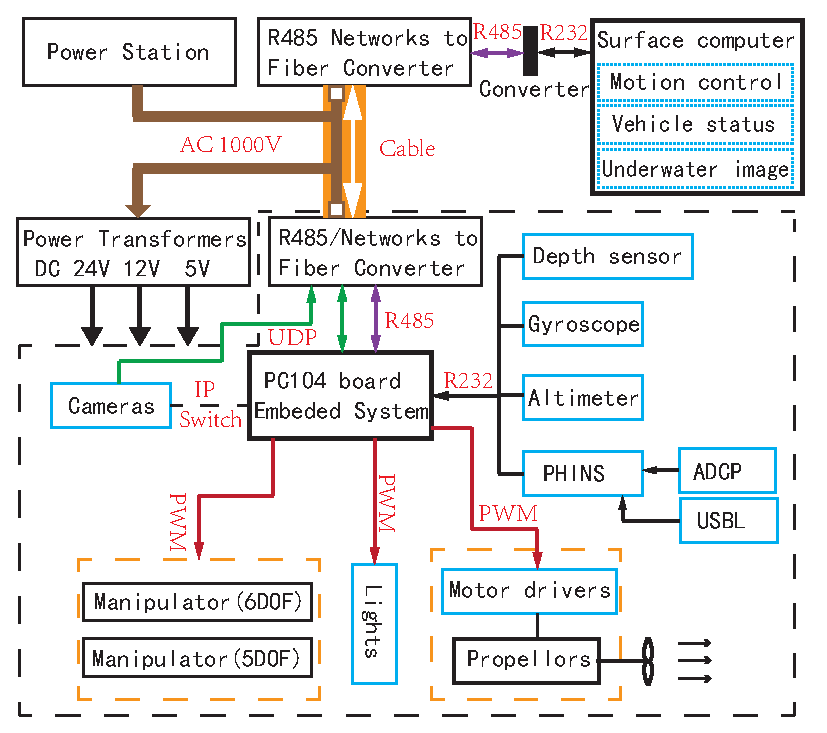
\includegraphics[width=14cm]{figure/chap2/F3.eps}
%\captionsetup{justification=centering}
\label{fig:chap2:F5}
\bicaption[fig:chap2:F5]{ROV 的系统控制框图}{ROV 的系统控制框图}{Fig.}{Diagram for ROV control system}
\end{figure}


\subsubsection{具有复杂形状的水下机器人数学模型 }

A. SJ-ROV 概况

SJ-ROV 3000 水下机器人是一款深海工作的ROV,其前置有两个机械手,可用作控制理论、水下科考等研究的实验平台。该型水下机器人由上海交通大学开发,具有多种工作模式,能够接受期望指令,并进行高精度导航寻迹控制\cite{lekkas2013line}。此外,当ROV的动力定位模式被打开时,该型水下机器人也可用来采集水下样本等。不同于海龙二号ROV\cite{xu2005deeprov,Huo2016Impulse},该型水下机器人推进器是电机驱动。机器人的关键部件,如压力舱体、动力系统、通信系统已经完成了测试,可以确保机器人工作的安全性与可靠性。目前,在一个最大深度为11m,长度为10m,宽度为6m的室内实验池内完成了初次航行实验\ref{fig:chap2:F3}。水下机器人的外形见图\ref{fig:chap2:F1},关键参数可以参考列表\ref{T2:chap2}。


B. 观测与通信系统介绍

SJ-ROV 3000由于设计目标为水下3000米,属于海况未知且复杂的环境,为了提高水下机器人的工作性能与定位能力,装载了诸多高性能的传感器,以期实现水下高性能航行的实验目标。在本部分,传感器的安装位置如图\ref{fig:chap2:F4}已经被标示出。表\ref{T3:chap2}列出了该型ROV水下机器人上安装的传感器的名称与类型。为便于进行系统理解,水下机器人的控制与通信框图也在本部分给出,见图\ref{fig:chap2:F4}。在惯性测量单元(INS)、多普勒测速仪(APDL)、深度计等这些传感器的帮助下,可以采集到ROV的姿态位置、速度以及深度的测量信息。并且,该型水下机器人配置有前、后视觉摄像头、水下灯、两个机械手以及用于和水面控制台通信的超短基线模块(USBL)。


该型ROV是由岸上供电,通过使用电源转换模块,经过动力缆给水下设备供电。通信和控制的测试是在实验水池完成的,水密性和动力也均被测试。控制测试是采用RS-485协议来发送命令,通过水下缆线中的光纤,将命令成功地发送到水下航行器上。图像观测和数据采集也通过光纤被采集并显示到水面控制台的显示器上。

C. 建模

根据ROV的推进器布置示意图\ref{fig:chap2:F4},可以确定该型ROV有7个推进器,当水下机器人处于完全在水里的状态时,在各个自由度上均有直接的推进器推力,也就是ROV系统可以拥有任何自由度的瞬间加速度,${rank}[\bm{f}_2(\bm{q},{\dot{\bm{q}}},t)]=dim[\bm{q}] =6$, 因此该系统的控制输入是不小于系统自由度数目的。

Fossen提出的6自由度的水下机器人动力学模型是非线性的,可用于对该型ROV的模型简化。ROV的自重较大,因此水下机器人推重比(最大推力/重量)较小,使得水下机器人的模型对于环境与模型中的动态变化并不敏感。配载的传感器变化以及流体阻力带来的影响对于水下机器人的控制而言并不明显。因此,在对ROV进行建模的时候,需对Fossen提出的模型做简化处理。

\begin{equation}
\label{eq:5}
\bm{M} \bm{\dot \nu} + \bm{D} \bm{\nu} =  \bm {\tau }
\end{equation}
式中,惯性质量矩阵$\bm{M}$ 可以使用机械设计软件求出。航行器受到的阻力,很难进行实际测定。简化会主要考虑流体阻尼。一般使用流体力学软件模拟求出阻尼力项$\bm{D}$。由于水下机器人是ROV工作模式,运行速度足够小,因此,受到的阻力主要是非线性项。其余力学影响,在建模时很难被求解出来,一般作为模型不确定性和干扰来应对。

工程控制实践中为了方便以及减少建模的困难,常常采用PID方法来设计控制器,会将恢复力(矩)、流体阻力、科氏力及产生阻力、附加质量以及环境和动力缆中的干扰力等均不进行建模,而是通过使用PID控制器计算期望状态与实际状态的误差,将PID控制器的输出值分配给不同的推进器上,从而实现控制的目的。具体的方法在本章\ref{2_3}节中给出。


\subsubsection{鱼雷型水下机器人数学模型  }

通过理论分析和经验数据获得的REMUS 100 AUV的6自由度非线性系统模型是为改进REMUS的控制提供了更精确的机器人平台模型。在本节中将对REMUS 100 AUV进行模型与配置详细介绍。REMUS的坐标系以及模型外观示意如图\ref{fig:chap2:F6},图中各个参数量的表示可以参考表\ref{tab:chap2:notation}。该型水下机器人仅仅拥有一个螺旋桨推进器固定在尾部,有四个舵片,一对水平舵,一对垂直舵,以十字形式固定在尾部推进器的周围。由于REMUS工作的控制是具有6个自由度的,而只有3个驱动器,因此REMUS AUV是系统控制输入是小于系统自由度的,控制难度高。

 \begin{figure}[!htp]
 \centering
 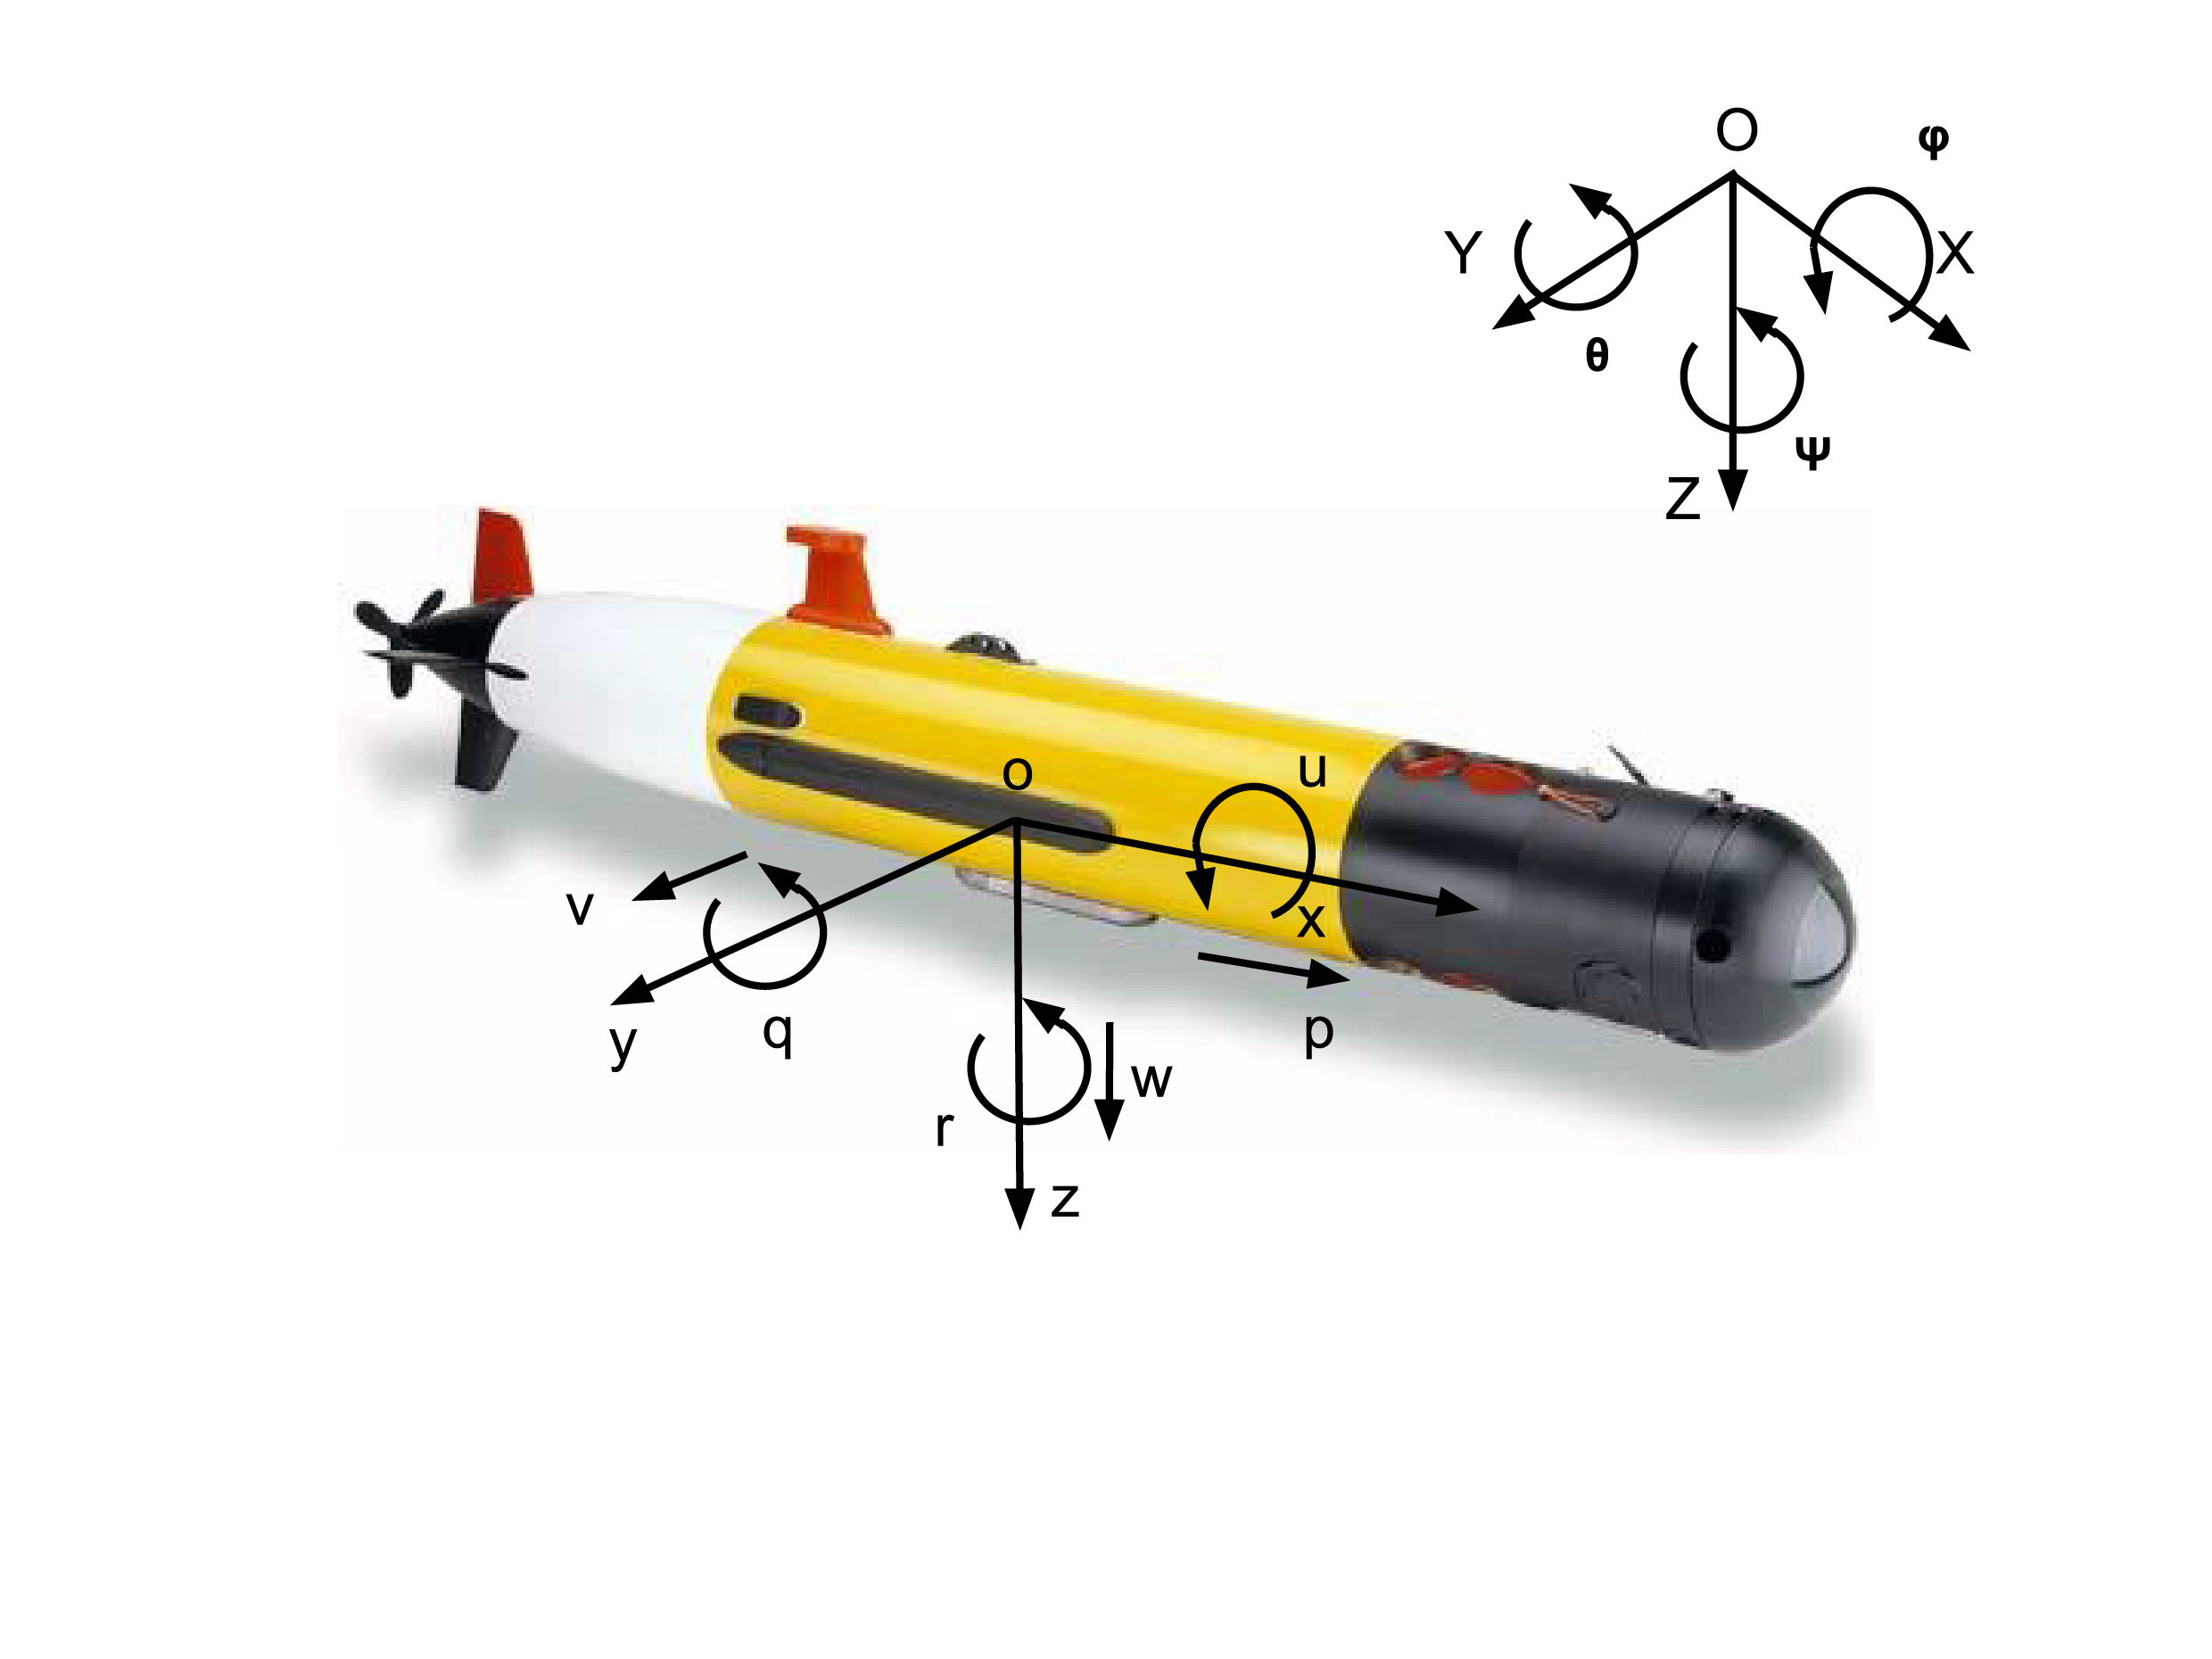
\includegraphics[width=11cm]{figure/chap2/REMUS_paper-300ppi.png}
 \label{fig:chap2:F6}
 \bicaption[fig:chap2:F6]{REMUS模型以及体坐标系、惯性坐标系示意}{REMUS模型以及体坐标系、惯性坐标系示意} {Fig}{REMUS body frame and inertial reference frame\cite{wu2016parametric}}
 \end{figure}

REMUS 100 AUV的体坐标系原点位于几何中心上,因此浮心与几何中心重合。重心略低于浮心,处于靠下的位置。REMUS航行器的模型也可使用Fossen提出的非线性模型。左侧为刚体动力学,右侧为外部作用力和力矩。前面已经讨论了B-frame原点与浮心重合的情况,这样REMUS模型的左侧刚体动力学可以使用式\ref{eq:chap2:16}的形式。由于REMUS中的驱动器有舵片和推进器两种,舵片和航行器本体存在力学耦合,要建立其模型相对复杂。Prestero\cite{prestero2001verification} 使用实验中的测量数据建立REMUS的精确非线性模型,该模型中AUV的强非线性、多自由度耦合性以及系统静不稳定特点都反映了出来,具有很大贡献。

由水下机器人的重力和浮力而产生的流体静力、舵片驱动器产生的控制力,附加质量、流体动力学力以及推进器产生的推力和扭矩都被包含在REMUS的6自由度非线性模型里面。考虑到上述的力和力矩,结合式\ref{eq:chap2:30}给出REMUS的各个自由度方程如下:
纵荡(Surge):
\begin{equation}
\label{eq:chap2:surgeremus}
\begin{aligned}
m &\left[ \dot u - vr  + wq - {x_G}({q^2} + {r^2}) + {y_G}(pq - \dot r) + {z_G}(pr + \dot q) \right] =  \\
&- (W - B)\sin \theta  + {X_{u\left| u \right|}}u\left| u \right| + {X_{\dot u}}\dot u + {X_{wq}}wq\\
&+ {X_{qq}}qq + {X_{vr}}vr + {X_{rr}}rr + {X_T}  \\
\end{aligned}
\end{equation}
横荡(Sway):
\begin{equation}
\label{eq:chap2:swayremus}
\begin{aligned}
 m&\left[ {\dot v - wp + ur - {y_G}({r^2} + {p^2}) + {z_G}(qr - \dot p) + {x_G}(qp + \dot r)} \right] =\\
 & (W - B)\cos \theta \sin \varphi  + {Y_{v\left| v \right|}}v\left| v \right| + {Y_{r\left| r \right|}}r\left| r \right| + {Y_{\dot v}}\dot v + {Y_{\dot r}}\dot r \\
 &+ {Y_{ur}}ur + {Y_{wp}}wp + {Y_{pq}}pq +  {Y_{uv}}uv + {Y_{uu\delta }}{u^2}{\delta _r}  \\
\end{aligned}
\end{equation}
垂荡(Heave):
\begin{equation}
\label{eq:chap2:heaveremus}
\begin{aligned}
 m&\left[ {\dot w - uq + vp - {z_G}({q^2} + {p^2}) + {x_G}(rp - \dot q) + {y_G}(rq + \dot p)} \right] =\\
 & (W - B)\cos \theta \cos \varphi  + {Z_{w\left| w \right|}}w\left| w \right| + {Z_{q\left| q \right|}}q\left| q \right| + {Z_{\dot w}}\dot w \\
 &+ {Z_{\dot q}}\dot q + {Z_{uq}}uq + {Z_{vp}}vp + {Z_{rp}}rp + {Z_{uw}}uw + {Z_{uu\delta }}{u^2}{\delta _e}  \\
\end{aligned}
\end{equation}
横滚(Roll):
\begin{equation}
\label{eq:chap2:rollremus}
\begin{aligned}
 {I_x}\dot p + &({I_z} - {I_y})qr + m[{y_G}(\dot w - uq + vp) - {z_G}(\dot v - wp + ur)] = \\
 &({y_G}W - {y_B}B)\cos \theta \cos \varphi  - ({z_G}W - {z_B}B)\cos \theta \sin \varphi \\
 & + {K_{p\left| p \right|}}p\left| p \right| + {K_{\dot p}}\dot p + {K_{prop}}  \\
\end{aligned}
\end{equation}
俯仰(Pitch):
\begin{equation}
\label{eq:chap2:pitchremus}
\begin{aligned}
 {I_y}\dot q + &({I_x} - {I_z})rp + m[{z_G}(\dot u - vr + wq) - {x_G}(\dot w - uq + vp)] = \\
 &- ({z_G}W - {z_B}B)\sin \theta  - ({x_G}W - {x_B}B)\cos \theta \cos \varphi  \\
 &+ {M_{w\left| w \right|}}w\left| w \right| + {M_{q\left| q \right|}}q\left| q \right|
  + {M_{\dot w}}\dot w + {M_{\dot q}}\dot q  + {M_{uq}}uq \\
   &+ {M_{vp}}vp +{M_{rp}}rp + {M_{uw}}uw + {M_{uu\delta }}{u^2}{\delta _e} \\
\end{aligned}
\end{equation}
偏航(Yaw):
\begin{equation}
\label{eq:chap2:yawremus}
\begin{aligned}
 {I_z}\dot r + &({I_y} - {I_x})pq + m[{x_G}(\dot v - wp + ur) - {y_G}(\dot u - vr + qw)] = \\
 &({x_G}W - {x_B}B)\cos \theta \sin \varphi  - ({y_G}W - {y_B}B)\sin \theta  \\
 &  + {N_{v\left| v \right|}}v\left| v \right| + {N_{r\left| r \right|}}r\left| r \right|  + {N_{\dot v}}\dot v  + {N_{\dot r}}\dot r + {N_{ur}}ur \\
 &  + {N_{wp}}wp  + {N_{uv}}uv + {N_{pq}}pq + {N_{uu\delta }}{u^2}{\delta _r} \\
\end{aligned}
\end{equation}
式中,各个系数都是使用REMUS的水池实验数据推导出的。每个系数的具体解释可以参考Prestero的论文附录\cite{prestero2001verification}。其中, $X_{u\left| u \right|}, X_{\dot u}, X_{wq},X_{vr},X_{qq}, X_{rr}$ 是x方向的阻力、附加质量系数。同样,在上面的公式中可以给出别的自由度的流体阻力和附加质量系数。需要注意的是,$Y_{ur},Z_{uq},N_{ur},M_{uq}$ 表示的是附加质量和舵片力的合力作用。$ M_{uw},N_{uv},Y_{uv},Z_{uw}$ 是考虑舵片升降力、体升降力及转矩的力学系数。 $Y_{uu\delta },Z_{uu\delta },N_{uu\delta},M_{uu\delta },X_T,K_{prop}$ 是与控制舵片和推进器有关的流体动力学系数。

\section{推进器布置与推力控制向量 }
\label{2_3}
\subsection{推进器布置 }
\subsubsection{常见的布置 }

对于水下机器人常用的推进器是:
一. 可旋转方向推进器:该类型驱动器可以绕固定推进器的轴(z-axis)旋转以产生不同的推力,在推进器的体坐标x-y平面内都可以产生推力$(F_x,F_y)$。这种类型的推进器有很大的优势,因其可以减少整体设备的功率,也适用更多的可能情况。不过,这种类型的推进器由于机械结构复杂增加了控制的复杂性与难度。
二. 固定式推进器:固定方向的推进器因其推进器的中轴线相对于水下机器人本体夹角固定而定义。因这种类型的推进器是提前固定好的,不能随着任务的变化而调整。本章重点分析这种推进器。
三. 槽道推进器:这种推进器是放置在水下机器人的壳体通道内,可以进行正反旋转,产生推力。这种推进器多用在形状有要求的水下机器人中。
四. 控制面:控制面多使用舵片,可以固定在不同的位置以产生升降力和阻尼力,这种控制面和鳍类似,可以用于俯仰,偏航等运动中。

\begin{figure}[h]
    \centering
        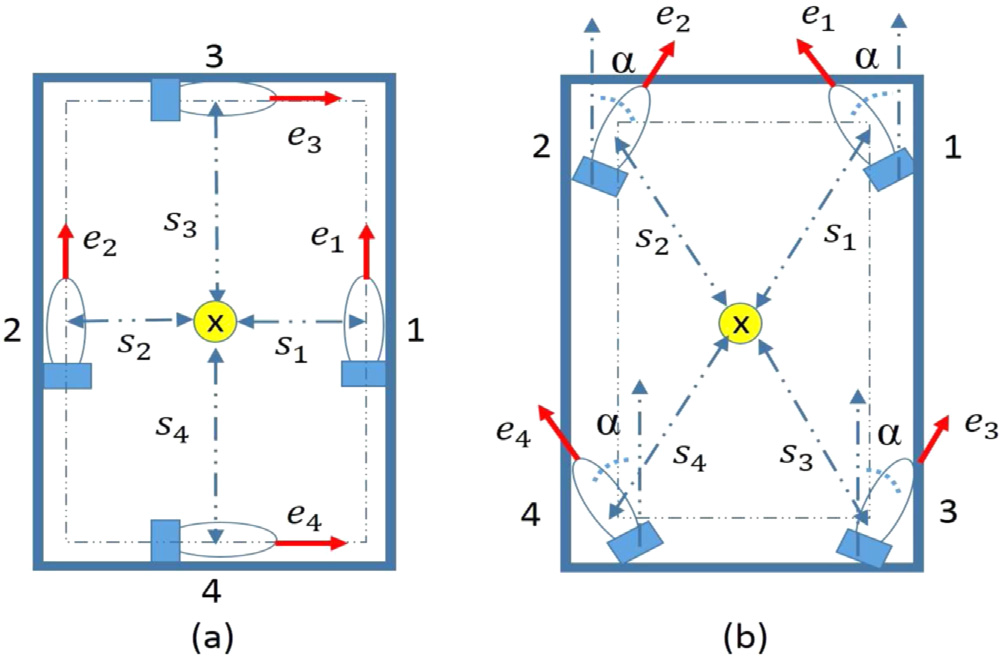
\includegraphics[width=12cm]{figure/chap2/configure.jpg}
        \label{fig:chap2:F7}
        \bicaption[fig:chap2:F7]{推进器的布置形式:左图:十字形式;右图:X 形式}{推进器的布置形式:左图:十字形式;右图:X 形式} {Fig}{Thruster configuration of vehicle: cross-shaped configuration(Left) and X-shaped configuration(right)}
\end{figure}

本工作将展示几种不同的推进器布置,这些是商业和科研水下机器人经常用的布置形式。在水下机器人的水平运动面内,有两种形式,十字形式和 X 形式, 如图\ref{fig:chap2:F7}\cite{dos2016bank}。十字形推进器布置又称为轴向布置,优点是该种布置形式下各个自由度的运动耦合性小。X形式布置又被称为矢量布置,它的优点是可以实现水平面内的各个自由度的运动控制。

水下机器人有很多种功用,也因此会衍生出很多个推进器布置形式,除了文中的布置形式还有如图\ref{fig:chap2:F8}所示的布置形式\cite{ardusub}。图中a和c图都是具有6个自由度的运动,推进器布置所提供的控制输入是不小于系统自由度数目的,且两种布置形式分别是从X形状和十字形状变化而来。b和d图中分别是5自由度和3自由度布置形式,b图中的布置经常用于水下机器人中,具有很好的推进器性能和灵活性;d图中的布置经常用于小型水下无人中,使用的推进器少,结构简单,可满足使用的基本功能要求。

\begin{figure}
%\begin{tabular}{cc}
\begin{minipage}{0.48\linewidth}
  \centerline{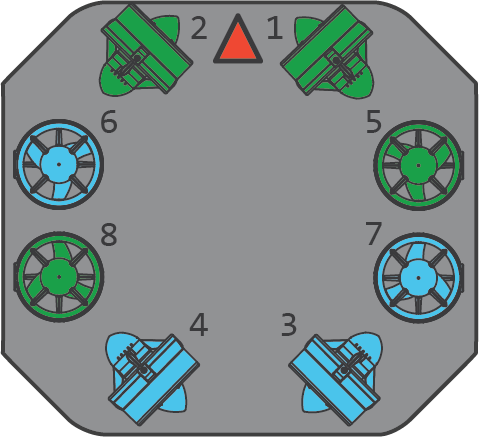
\includegraphics[width=4.0cm,height = 5cm]{figure/chap2/vectored6dof-frame.png}}
  \centerline{(a) 载重6自由度作业型布置}
\end{minipage}
\hfill
\begin{minipage}{.48\linewidth}
  \centerline{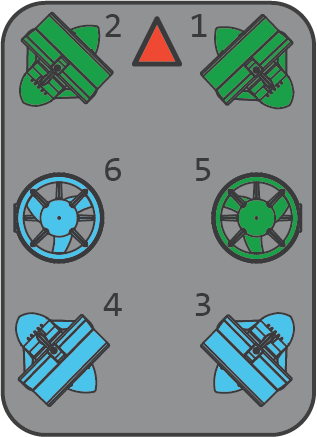
\includegraphics[width=4.0cm,height = 5cm]{figure/chap2/vectored-frame.png}}
  \centerline{(b) 5自由度布置}
\end{minipage}
\vfill
\begin{minipage}{0.48\linewidth}
  \centerline{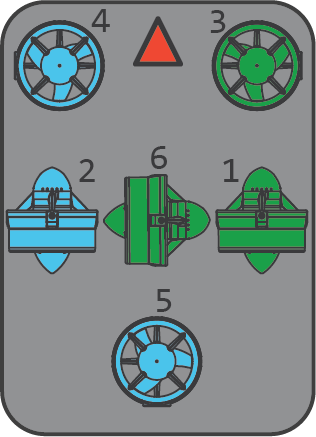
\includegraphics[width=4.0cm,height = 5cm]{figure/chap2/bluerov-frame.png}}
  \centerline{(c) 6自由度定位型布置}
\end{minipage}
\hfill
\begin{minipage}{0.48\linewidth}
  \centerline{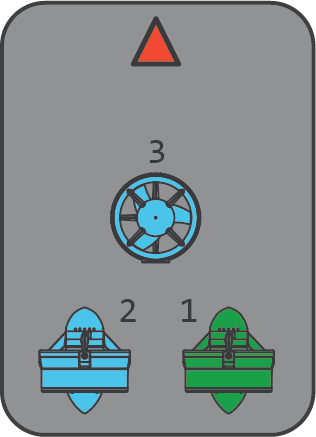
\includegraphics[width=4.0cm,height = 5cm]{figure/chap2/simplerov-3.png}}
  \centerline{(d) 3自由度布置}
\end{minipage}
%\end{tabular}
\label{fig:chap2:F8}
\bicaption[fig:chap2:F8]{水下机器人常用布置}{水下机器人常用布置} {Fig}{Congfiguration used in vehicle mostly\cite{ardusub}}
\end{figure}

\subsubsection{推力分配模型 }
电动螺旋桨推进器常常被用来驱动水下机器人。根据推进器布置的方式,这些推进器被划分为水平螺旋桨  $T_H$和垂直螺旋桨 $T_V$。正如图\ref{fig:chap2:F4}所示的一种形式,图中有四个水平置螺旋桨推进器 ,分别被图中标号为1, 2, 3, 4。图中5, 6, 7标识的为垂直放置推进器。水下推进器安装也有多种形式,对于SJ-3000 ROV, 水平推进器布置是X形式,这样可以提高推进器在水平面内的控制便捷性。中间的两个垂直推进器之间有夹角,也便于调节ROV的横滚运动。因此,本文给出推进器的布置形式与水下机器人的受力和力矩的数学关系如下\cite{dos2016bank}:

\begin{equation}
\label{eq:chap2:thrustconfigure_1}
  \begin{array}{l}
   {\bm \tau} = \bm{BT} \\
  \end{array}
\end{equation}
式中,$\bm{B}$表示螺旋桨推进器的布置矩阵,$\bm{T}$ 表示各推进器的推力组成的向量,向量的长度为推进器的个数$N$。对于文中的3000m的ROV,推力向量$\bm{T} = [T_1,T_2,T_3,T_4,T_5,T_6,T_7]^T$。$\bm{B}$ 是6*N的矩阵,且一般情况下,布置矩阵不是方阵。

为了更方便描述水下机器人的运动,常常会将6自由度的运动分为水平面运动和垂直面运动。因此,水下机器人受到推力$\bm \tau$也可以分为水平面合力 $\tau_H$ 和垂直面合力 $\tau_V$,这些力都是由推进器产生,但会对因为所处的运动不同,而在不同的运动面内对水下机器人的力学效果也有所差异。同样,\\
\begin{eqnarray}
\label{eq:chap2:BvBh}
\centering
T &=& \left[ {\begin{array}{*{20}{c}}
   {{T_H}}  \\
   {{T_V}}  \\
\end{array}} \right]\\
B &=& [\begin{array}{*{20}{c}}
    {{B_H}} & {0_{3\times3}}  \\
    {0_{3\times4}} & {{B_V}}  \\
\end{array}]
\end{eqnarray}
是根据推进器布置情况和运动面定义的推进器推力向量与分布矩阵。对于文中的ROV,$T_H = [T_1, T_2, T_3, T_4]^T$, $T_V = [T_5,T_6,T_7]^T$ 分别为水平面、垂直面的有贡献的推进器的推力。

确定了单个推进器推力以及推进器与运动的关系,可给出ROV的六个自由度方向上的推力分配方程。
\begin{equation}
\label{eq:chap2:thrustconfigure_2}
     \left[ \begin{array}{*{20}{c}}
     \tau_H\\
     \tau_V\\
     \end{array}\right]
      =
     [\begin{array}{*{20}{c}}
     {{B_H}} & {0_{3\times3}}  \\
     {0_{3\times4}} & {{B_V}}  \\
     \end{array}]\left[ {\begin{array}{*{20}{c}}
     {{T_H}}  \\
     {{T_V}}  \\
     \end{array}} \right] \\
\end{equation}
式中,$\tau_H = [\tau_{surge},\tau_{sway},\tau_{yaw}]^T$ 和 $\tau_V=[\tau_{heave},\tau_{pitch},\tau_{roll}]^T$。需要注意的是,水平面和垂直面的划分因水下机器人而异,本文的建立的推力分配矩阵是以3000m ROV为例,进行的分析。

本文中的推进器是由无刷直流电机带动螺旋桨而产生推力,该电机的最大转速是1850 $rpm$。推进器的推力线性特性较好,大大减轻了推进器性能差而控制困难的问题。推进器的模型是通过敞水实验获得的,参考模型是公式\ref{eq:chap2:29},但由于推进器正反推力最大值不同,获得推进器模型如下\cite{wunl2011immune}:

\begin{equation}
\label{eq:8}
{T_i} = \left\{ {\begin{array}{*{20}{c}}
   {{\gamma _1}{n^2}} & {if}  \\
   {{\gamma _{^2}}{n^2}} & {if}  \\
\end{array}} \right.\begin{array}{*{20}{c}}
   {{T_{i - }}_{\max } = 120kgf} & {forward}  \\
   {{T_{i - }}_{\max } = 90kgf } & {reverse}  \\
\end{array}
\end{equation}
式中 $\gamma _1 > 0$ 和 $\gamma _2 < 0$ 为推进器的正反推力系数;$n$为推进器电机转速。

应当指出的是螺旋桨推进器的叶片有逆时针和顺时针两种,这两种叶片也文中的ROV中成对使用,以便互相抵消扭矩。

\subsection{推力控制向量 }
\subsubsection{定义}
传统的推力分配时,等式\ref {eq:chap2:thrustconfigure_1}和\ref{eq:chap2:thrustconfigure_2}经常通过使用$\bm{B}$的伪逆矩阵来求解各推进器上的推力分布。然而,本文中的例子ROV,用于控制深度的螺旋桨推进器有三个,但并不总是每个推进器都是最佳选择,例如靠近ROV尾部的第七螺旋桨 $T_7$ 。实际上,使用 $T_5$ 和 $T_6$ 将更好地解决的深度控制问题。此外,有时需要根据ROV的功能来修改螺旋桨的布置形式,因此计算的布置矩阵会因某个推进器的变化而整体受影响,这对于系统的稳定并不是好的方案。单个推进器因布置位置的不同而可能对水下机器人的每个自由度的运动产生影响,那么是否可以考虑对单个推进器在整体运动中的作用来描述单个推力与整体运动所需控制力的关系呢?首先,要确定要描述推进器对每个自由度的影响的数学方程。本文提出使用推力控制向量来表征运动和推力的关系。一般在状态反馈控制中,ROV受到的实际力是不可以测量的,而是通过姿态传感器的实际值与期望值进行对比,将反馈误差输入控制器,控制器的输出便是$\bm{\tau_{Desired} }$,就是期望的合推力。而推力分配矩阵的最大目的就是将$\bm{\tau_{Desired} }$ 有效地分配给各个有关的推进器,但用于控制的推力控制向量与运动学的描述并不相同,该向量面向于控制而非数学中的力分配。推力控制向量如下\cite{ardupilot,ardusub}:
\begin{equation}
\label{eq:chap2:motor_factor}
\bm{\beta}_{i}=
\left[
\begin{array}{*{20}{c}}
  {f}_{surge}\\
  {f}_{sway}\\
  {f}_{heave}\\
  {f}_{roll}\\
  {f}_{pitch}\\
  {f}_{yaw}\\
\end{array}
\right]
\end{equation}
式中,$i$表示第 $i$ 个推进器。向量从上到下依次为电机纵荡系数(MOT SURGE FACTOR)、电机横荡系数(MOT SWAY FACTOR)、电机垂荡系数(MOT HEAVE FACTOR)、电机横滚系数(MOT ROLL FACTOR)、电机俯仰系数(MOT PITCH FACTOR)、电机偏航系数(MOT YAW FACTOR)。

因此,即使螺旋桨的布置发生变化,可通过将螺旋桨的推力控制矢量加入(Add)或删除(Delete)到ROV控制系统的推进器加载系统中进行推进系统快速升级,也可以合理地设定各个螺旋桨的推力控制向量中的各个自由度运动的有效力系数,而不必影响原有的控制方法以及其他推进器,如代码\ref{thrustercode:chap2}。在下一部分中,每个推进器的系数将根据控制模式设置并构成新的推力分布矩阵。\\

\begin{lstlisting}[language={C}, caption={ROV的推力布置示例\label{thrustercode:chap2}}][b]
static Thruster SJ_ROV_3000[] ={
       Thruster(0, MOT_1_SURGE_FACTOR, MOT_1_SWAY_FACTOR, MOT_1_HEAVE_FACTOR, MOT_1_ROLL_FACTOR, MOT_1_PITCH_FACTOR, MOT_1_YAW_FACTOR),
       Thruster(1, MOT_2_YAW_FACTOR, MOT_2_SURGE_FACTOR, MOT_2_SWAY_FACTOR, MOT_2_HEAVE_FACTOR, MOT_2_ROLL_FACTOR, MOT_2_PITCH_FACTOR),
       Thruster(2, MOT_3_SURGE_FACTOR, MOT_3_SWAY_FACTOR, MOT_3_HEAVE_FACTOR, MOT_3_ROLL_FACTOR, MOT_3_PITCH_FACTOR, MOT_3_YAW_FACTOR),
       Thruster(3, MOT_4_SURGE_FACTOR, MOT_4_SWAY_FACTOR, MOT_4_HEAVE_FACTOR, MOT_4_ROLL_FACTOR, MOT_4_PITCH_FACTOR, MOT_4_YAW_FACTOR),
       Thruster(4, MOT_5_SURGE_FACTOR, MOT_5_SWAY_FACTOR, MOT_5_HEAVE_FACTOR, MOT_5_ROLL_FACTOR, MOT_5_PITCH_FACTOR, MOT_5_YAW_FACTOR),
       Thruster(5, MOT_6_SURGE_FACTOR, MOT_6_SWAY_FACTOR, MOT_6_HEAVE_FACTOR, MOT_6_ROLL_FACTOR, MOT_6_PITCH_FACTOR, MOT_6_YAW_FACTOR),
       Thruster(6, MOT_7_SURGE_FACTOR, MOT_7_SWAY_FACTOR, MOT_7_HEAVE_FACTOR, MOT_7_ROLL_FACTOR, MOT_7_PITCH_FACTOR, MOT_7_YAW_FACTOR)
}
\end{lstlisting}

\subsubsection{PID控制应用实例 }
水下机器人的姿态控制是水下机器人控制中很重要的一项,一般是通过姿态角的依次控制来实现追踪期望命令。在刚刚接到控制命令时,首先要调整偏航角,这个阶段偏航角与俯仰角控制器不接收新的命令,以防止耦合影响。其次是调整俯仰角度,这时偏航角和横滚角度控制器不接收新的控制命令。最后是调节横滚角度。该种姿态控制方法经常被用于无人机上,可以通过使用PID控制器来完成高性能的任务\cite{mellinger2012trajectory}。水下机器人姿态控制器给出如下:

\begin{equation}
\label{eq:11}
\begin{array}{l}
 \Delta \varphi  = {k_{p,\varphi }}{e_\varphi } + {k_{i,\varphi }}\int {{e_\varphi }dt}  + {k_{d,\varphi }}{{\dot e}_\varphi } \\
 \Delta \theta  = {k_{p,\theta }}{e_\theta } + {k_{i,\theta }}\int {{e_\theta }dt}  + {k_{d,\theta }}{{\dot e}_\theta } \\
 \Delta \psi  = {k_{p,\psi }}{e_\psi } + {k_{i,\psi }}\int {{e_\psi }dt}  + {k_{d,\psi }}{{\dot e}_\psi } \\
 \end{array}
\end{equation}
式中,$k_p,k_i, k_d$为PID控制的控制参数。$\Delta \varphi, \Delta \theta, \Delta \psi$ 为PID输出的矫正力。

通过分析每个螺旋桨推进器的现有安装形式下水下机器人运动受到的力学影响,确定出推进器对每个姿态角的方向上的推力控制向量的系数。将获得的各推力控制向量进行组合,并将PID控制器的反馈矫正力分配到合适的推进器上,给出的计算公式如下:

\begin{equation}
\label{eq:12}
\left[ {\begin{array}{*{20}{c}}
   {{T_1}_{CMD}}  \\
   {{T_2}_{CMD}}  \\
   {{T_3}_{CMD}}  \\
   {{T_4}_{CMD}}  \\
   {{T_5}_{CMD}}  \\
   {{T_6}_{CMD}}  \\
   {{T_7}_{CMD}}  \\
\end{array}} \right] = \left[ {\begin{array}{*{20}{c}}
   0 & 0 & 1  \\
   0 & 0 & { - 1}  \\
   0 & 0 & { - 1}  \\
   0 & 0 & 1  \\
   1 & 0 & 0  \\
   { - 1} & 0 & 0  \\
   0 & 1 & 0  \\
\end{array}} \right]\left[ {\begin{array}{*{20}{c}}
   {\Delta \varphi }  \\
   {\Delta \theta }  \\
   {\Delta \psi }  \\
\end{array}} \right]
\end{equation}
其中公式\ref{eq:12}右边为推力控制向量矩阵与PID反馈的矫正力。推力控制向量矩阵的第\textit{i}行分别为第\textit{i}个推进器对姿态的各个自由度的力学系数。因为PID控制器的系数也是可以调节的,因此在推力控制向量中的系数可以定义为1, 0 , -1。

本节建立了推进器和控制器之间的推力分配关系,该分配关系可以选出对所需控制的运动最有效的推进器,如此ROV可以跟踪所要求的方向指令,并完成状态调整。

\section{本章小结 }

本章系统地引入了一般形式的水下机器人的坐标系、运动学状态转换方程、流体动力学模型,便于水下机器人进行后续的模型参数计算和控制应用;分析文中研究的两种不同外形的水下机器人,首先给出具有非初等几何外形的水下机器人的数学描述,而后给出该型水下机器人的简化模型;给出了鱼雷形状的水下机器人的数学模型,并分析了系统需要关注的系统动态特性。最后,根据推进器的空间布置,给出了不同形式的推力分配模型。分析建立的基于运动学的推力分配模型,提出面向控制的推力控制向量,着重利用对运动影响性强的推进器,并使用中水下机器人的PID姿态控制来进行实例化分析。
